\documentclass{article}


\usepackage{PRIMEarxiv}

\usepackage[utf8]{inputenc}
\usepackage[T1]{fontenc}
\usepackage{hyperref}
\usepackage{url}
\usepackage{booktabs}
\usepackage{amsfonts}
\usepackage{amsmath, amssymb}
\usepackage{enumitem}
\usepackage{nicefrac}
\usepackage{microtype}
\usepackage{graphicx}
\graphicspath{{media/}}
\usepackage{libertine}
\usepackage{libertinust1math}
\usepackage{dsfont}
\usepackage{nicefrac}
\usepackage{todonotes}



% Theorem environments
\usepackage{amsthm}  % For theorem-like environments
\theoremstyle{plain}
\newtheorem{theorem}{Theorem}
\newtheorem{lemma}[theorem]{Lemma}
\newtheorem{corollary}[theorem]{Corollary}
\newtheorem{proposition}[theorem]{Proposition}
\newtheorem{algorithm}[theorem]{Algorithm}
\newtheorem{assumption}[theorem]{Assumption}

\theoremstyle{definition}
\newtheorem{definition}{Definition}
\newtheorem{example}{Example}

\theoremstyle{remark}
\newtheorem{remark}{Remark}
    
\NewDocumentCommand{\br}{m}{\left( #1 \right)}
\NewDocumentCommand{\bs}{m}{\left[ #1 \right]}
\NewDocumentCommand{\bc}{m}{\left\{ #1 \right\}}

% Sets and number systems using dsfont (mathds)
\NewDocumentCommand{\R}{}{\mathds{R}}  % Real numbers
\RenewDocumentCommand{\H}{}{\mathds{H}}  % Hilbert space
\NewDocumentCommand{\N}{}{\mathds{N}}  % Natural numbers
\NewDocumentCommand{\Z}{}{\mathds{Z}}  % Integers
\NewDocumentCommand{\Q}{}{\mathds{Q}}  % Rational numbers
\NewDocumentCommand{\C}{}{\mathds{C}}  % Complex numbers
\NewDocumentCommand{\ind}{}{\mathds{1}}  % Complex numbers

% Mathematical operators and functions
\NewDocumentCommand{\defeq}{}{\coloneq} % Definition equal (
\NewDocumentCommand{\der}{}{\mathrm{d}}  % Differential oper
\NewDocumentCommand{\cder}{}{\partial}  % Differential oper
\NewDocumentCommand{\mul}{mm}{\langle #1, #2 \rangle}  % Inn
\NewDocumentCommand{\norm}{m}{\left\lVert #1 \right\rVert}  
\NewDocumentCommand{\abs}{m}{\left\lvert #1 \right\rvert}  %


\NewDocumentCommand{\maximize}{}{\text{maximize }}
\NewDocumentCommand{\minimize}{}{\text{minimize }}
\NewDocumentCommand{\subjectto}{}{\text{subject to }}
\NewDocumentCommand{\overall}{}{\text{over all }}


% Additional common mathematical abbreviations
\DeclareMathOperator*{\argmin}{arg\,min}
\DeclareMathOperator*{\argmax}{arg\,max}
\DeclareMathOperator{\dom}{dom}
\DeclareMathOperator{\epi}{epi}
\DeclareMathOperator{\prox}{prox}
\DeclareMathOperator{\conv}{conv}
\DeclareMathOperator{\tr}{tr} % Already using \operatorname,
\DeclareMathOperator{\rank}{rank} % Already using \operatorn

% More definitions as needed
\NewDocumentCommand{\grad}{}{\nabla}

\let\olddisplayopen\[
\let\olddisplayclose\]

% Redefine \[ and \]
\RenewDocumentCommand{\[}{}{%
  \begin{equation}\begin{aligned}%
}
\RenewDocumentCommand{\]}{}{%
  \end{aligned}\end{equation}%
}



%% Title
\title{Parametric Audio-Visual SELD via Variational Inference and Implicit Feature Pooling
%%%% Cite as
%%%% Update your official citation here when published 
\thanks{\textit{\underline{Citation}}: 
\textbf{Authors. Title. Pages.... DOI:000000/11111.}} 
}

\author{
  Bogdan Jastrzębski \\
  Samsung R\&D Institute Poland (SRPOL) \\
  Warsaw \\
  \texttt{b.jastrzebsk@samsung.com} \\
  \AND
  Rafał Foltyniewicz \\
  Samsung R\&D Institute Poland (SRPOL) \\
  Warsaw \\
  \texttt{r.foltyniewi@samsung.com} \\
  %% \And
  %% Coauthor \\
  %% Affiliation \\
  %% Address \\
  %% \texttt{email} \\
  %% \And
  %% Coauthor \\
  %% Affiliation \\
  %% Address \\
  %% \texttt{email} \\
}


\begin{document}
\maketitle


\begin{abstract}
Current sound event localization systems reconstruct dense spatial maps from 4-channel microphone arrays, an underdetermined inverse problem whose exact numerical solvers produce checkerboard artifacts that convolutional detection heads misinterpret as genuine sources. We propose a parametric approach: the microphone covariance is modeled directly as a superposition of steering vectors weighted by continuous Gaussian source parameters. Source locations are recovered by solving a nonlinear least squares problem over the parameter space, bypassing dense grid rendering entirely. At 14~$\mu$s per gradient step (analytical gradients, Adam), cold-start convergence completes in 4.2~ms (300 iterations), while warm-start temporal tracking requires under 100~$\mu$s per frame---a 350$\times$ speedup over the ADMM baseline. An \textbf{envelope theorem} formulation separates spatial fitting from classification: Gaussian parameters are treated as the solution of a per-frame $\operatorname{argmin}$, and training gradients flow through the classifier and feature pooling stages without backpropagating through the optimization itself. This decoupling enables independent optimization of the spatial and semantic objectives while maintaining end-to-end differentiability of the classification pathway.
\end{abstract}


\keywords{Sound Event Localization and Detection \and Covariance Matching \and Parametric Gaussians \and Envelope Theorem \and Implicit Feature Pooling}


\section{Introduction}
This is a proposal for research in audio source localization and classification in real-time audio-visual settings. The task is to detect sound sources from 4 microphone and 360$^\circ$ camera data, and classify them into specific classes (e.g., speech, alarm, vacuum cleaner, footsteps, dog bark, baby cry, crash, scream, door knock, phone ring, laughter, cat, blender). The challenge is to make the solution fast and possible to use in real-time on small devices. The proposal is directly inspired by the DCASE challenge.


\section{Probabilistic Model and Bayesian State Tracking}
Let $Y$ represent the true target variables. The true state of the acoustic environment at a frame consists of $M$ discrete point sources: $Y = \{ (s_m, c_m) \}_{m=1}^M$, where $s_m \in \Omega$ is the true physical coordinate and $c_m \in \{1, \dots, C\}$ is the categorical class label.

Because $s_m$ are unknown and the sensory data is ambiguous, we model our uncertainty using $K$ parametric Gaussians. The latent state at time $t$ is $\Theta^{(t)} = \{\mu_k^{(t)}, \pi_k^{(t)}\}_{k=1}^K$, where $\mu_k$ is the spatial centroid and $\pi_k$ the source intensity. We track these parameters via a recursive Bayesian filter:
\begin{equation}
p(\Theta^{(t)} \mid \mathcal{D}_{1:t}) \propto p(\mathcal{D}^{(t)} \mid \Theta^{(t)}) \, p(\Theta^{(t)} \mid \mathcal{D}_{1:t-1})
\end{equation}

The observation model $p(\mathcal{D}^{(t)} \mid \Theta^{(t)})$ is the spatial likelihood defined in Section~3. The temporal prior $p(\Theta^{(t)} \mid \mathcal{D}_{1:t-1})$ is formed by marginalizing over the previous frame's posterior, which effectively ``blurs'' the covariance of the previous estimate---anchoring the new Gaussians near their previous locations while allowing them to track moving subjects. In practice this is implemented as \textbf{warm-start}: parameters converge in 3--5 gradient steps from the previous frame's solution, compared to 300 from random initialization.


\section{Spatial Localization as a Nonlinear Least Squares Problem}

\subsection{Steering Vectors and Covariance}
Let $\mathbf{a}(\mu) \in \mathbb{C}^4$ denote the complex steering vector for a far-field point source at angular direction $\mu = (\theta, \phi)$, evaluated at the 4-channel Eigenmike subset:
\begin{equation}
a_i(\mu) = \exp\!\left(-i \frac{2\pi}{\lambda} \, \mathbf{r}_i \cdot \mathbf{s}(\mu)\right)
\end{equation}
where $\mathbf{s}(\mu) = (\cos\phi \cos\theta,\; \cos\phi \sin\theta,\; \sin\phi)$ is the unit direction vector, $\mathbf{r}_i \in \mathbb{R}^3$ are the microphone positions (planar ring, radius 42~mm), and $\lambda$ is the acoustic wavelength at the center frequency ($\approx$4833~Hz). Each source contributes a rank-1 term to the observed $4 \times 4$ covariance matrix $C_{\text{obs}}$ via the outer product $\mathbf{a}(\mu_k) \mathbf{a}(\mu_k)^H$. The predicted covariance is:
\begin{equation}
C_{\text{pred}}(\Theta) = \sum_{k=1}^K \pi_k \; \mathbf{a}(\mu_k) \mathbf{a}(\mu_k)^H
\end{equation}

\subsection{Optimization Problem}
The spatial fitting objective minimizes the Frobenius norm between predicted and observed covariance:
\begin{equation}
\boxed{\Theta^* = \argmin_{\Theta}\; \mathcal{L}_{\text{spatial}}(\Theta) \;=\; \argmin_{\Theta}\; \big\| C_{\text{obs}} - C_{\text{pred}}(\Theta) \big\|_F^2}
\end{equation}
This is a \textbf{nonlinear least squares} problem: smooth ($C^\infty$, since steering vectors are sines and cosines of dot products), but non-convex due to periodicity in azimuth and permutation symmetry of the $K$ Gaussians. The 4-mic planar array exhibits front-back ambiguity ($\mu$ and its opposite hemisphere copy produce identical covariance), an inherent limitation resolved by the visual stream.

\subsection{Analytical Gradients and Adam}
The gradient $\partial\mathcal{L}_{\text{spatial}} / \partial \mu_k$ follows analytically from the steering vector Jacobian:
\begin{equation}
\frac{\partial a_i}{\partial \theta} = -i \frac{2\pi}{\lambda} \, a_i \, (\mathbf{r}_i \cdot \partial\mathbf{s}/\partial\theta), \qquad
\frac{\partial a_i}{\partial \phi} = -i \frac{2\pi}{\lambda} \, a_i \, (\mathbf{r}_i \cdot \partial\mathbf{s}/\partial\phi),
\end{equation}
with $\partial\mathbf{s}/\partial\theta = (-\cos\phi \sin\theta,\; \cos\phi \cos\theta,\; 0)$ and $\partial\mathbf{s}/\partial\phi = (-\sin\phi \cos\theta,\; -\sin\phi \sin\theta,\; \cos\phi)$. The chain rule through the Frobenius norm yields per-source gradients. Parameters $\pi_k$ are parametrized in log-space for positivity, with the chain rule $\partial\mathcal{L}/\partial(\log\pi_k) = \partial\mathcal{L}/\partial\pi_k \cdot \pi_k$.

We use the \textbf{Adam} optimizer: per-parameter adaptive learning rates naturally handle the ill-conditioning across parameter scales ($\mu_k$ in radians $\sim 0$--$6$, $\pi_k$ spanning $\sim 10^{-2}$--$10$). A Gauss-Newton solver was attempted but the exponential nonlinearity in $\mathbf{a}(\mu)$ causes the linearized Jacobian to overshoot by $>2$~radians per step even with Levenberg-Marquardt damping (see Appendix~\ref{sec:gn}).


\section{Envelope Theorem: Differentiable Spatial Fitting}
\label{sec:envelope}

The full model architecture involves both spatial localization and semantic classification. The visual encoder $f_v$ (YOLO backbone) produces a feature field $H_v$, which is pooled around the estimated source locations $\mu_k$ to produce localized feature vectors $z_k$, then classified via a lightweight MLP head. The key challenge is that $\mu_k$ are themselves the \emph{solution} of an optimization problem:
\begin{equation}
\Theta^*(\varphi) = \argmin_{\Theta}\; \mathcal{L}_{\text{spatial}}(\Theta; \varphi)
\end{equation}
where $\varphi$ denotes the encoder parameters (YOLO weights). The spatial loss $\mathcal{L}_{\text{spatial}}$ is independent of $\varphi$---it depends only on the microphone covariance $C_{\text{obs}}$ and the steering vectors. Therefore the optimal $\Theta^*$ does not depend on $\varphi$ for the spatial task. However, the \emph{classification} loss $\mathcal{L}_{\text{cls}}$ depends on $\Theta^*$ through the feature vectors $z_k(\Theta^*)$.

By the \textbf{envelope theorem}, since $\nabla_\Theta \mathcal{L}_{\text{spatial}}(\Theta^*; \varphi) = 0$ at the optimum and $\mathcal{L}_{\text{spatial}}$ is independent of $\varphi$, the total derivative simplifies:
\begin{equation}
\frac{d\mathcal{L}_{\text{cls}}}{d\varphi} = \frac{\partial\mathcal{L}_{\text{cls}}}{\partial\varphi}
      + \cancel{\frac{\partial\mathcal{L}_{\text{cls}}}{\partial\Theta^*} \cdot \frac{d\Theta^*}{d\varphi}}
\end{equation}

The term $d\Theta^*/d\varphi = 0$ because the spatial objective depends only on the microphone data, not on the encoder weights. Consequently, gradients flow through the model as follows:
\begin{enumerate}[label={(\arabic*)}]
    \item Spatial fitting solves $\Theta^* = \argmin \mathcal{L}_{\text{spatial}}$ (3--300 Adam steps). The result is \textbf{detached} from the computation graph.
    \item Feature pooling computes $z_k = \int H_v(x)\,\mathcal{N}(x \mid \mu_k, \Sigma_k)\,dx$ (differentiable soft attention).
    \item Classification head outputs $\hat{c}_k = \text{Softmax}(W z_k + b)$.
    \item Backpropagation: $\partial\mathcal{L}_{\text{cls}} / \partial \varphi$ flows through the classifier and feature pooling into the YOLO backbone. No gradient flows through the spatial optimizer.
\end{enumerate}

This decoupling is both practical and theoretically sound: the spatial and semantic objectives are optimized independently, the classification pathway is fully differentiable, and the expensive $\operatorname{argmin}$ is never part of the backward pass.


\section{Experimental Validation}

\subsection{Spatial Localization}
We implemented the spatial fitting module in Julia using the 4-channel Eigenmike subset with analytical gradients and Adam (lr=$10^{-2}$). Per-iteration cost is \textbf{14~$\mu$s} (581 allocations, 31~KiB). Cold start converges in 300 iterations (\textbf{4.2~ms}), recovering both source directions to within 0.02~radians (NMSE 0.40). Warm-start temporal tracking requires 3--5 iterations (\textbf{$<$100~$\mu$s}), a 350$\times$ per-frame speedup over ADMM's 35~ms.

\begin{figure}[ht]
\centering
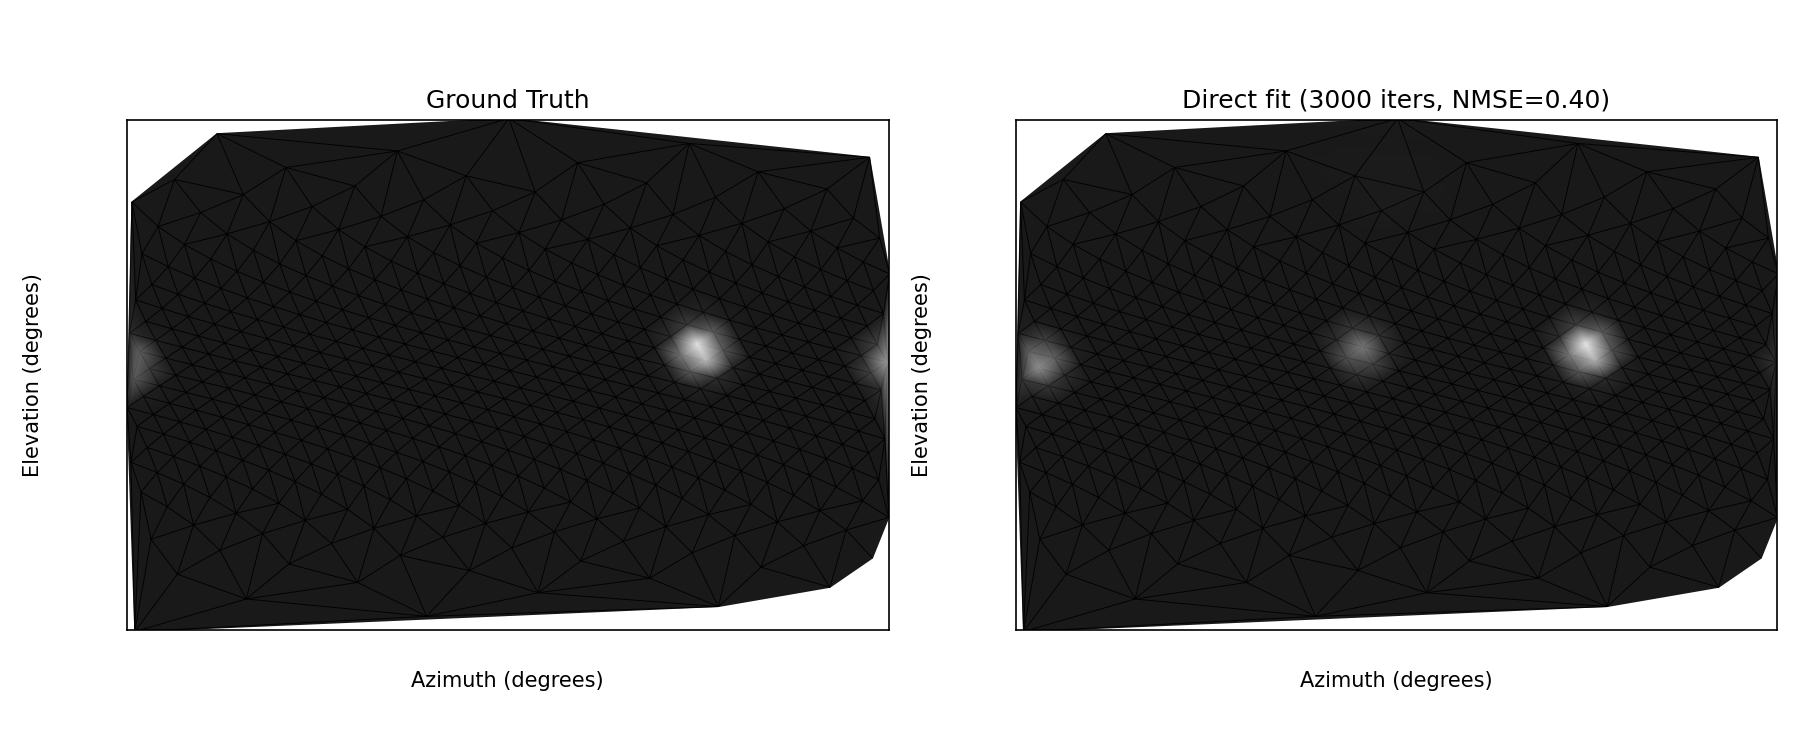
\includegraphics[width=\textwidth]{media/direct_fit_viz.png}
\caption{Spatial fitting result: ground truth (left) vs.\ fitted Gaussians (right) on synthetic 2-source data. NMSE = 0.40. The two true sources are recovered; residual Gaussians at opposite azimuth correspond to front-back ambiguous copies inherent to the 4-microphone planar array.}
\label{fig:direct_fit}
\end{figure}

\subsection{Architecture and Training}
The full model is implemented as a PyTorch module (\texttt{pytorch\_seld/}). The pipeline consists of: (1)~YOLO feature extraction (placeholder CNN backbone, 256 output channels), (2)~spatial fitting via Adam (300 cold / 5 warm iterations), (3)~implicit feature pooling over a $128 \times 256$ angular grid, (4)~classification head (MLP, 14 output classes). Training follows the envelope theorem protocol of Section~\ref{sec:envelope}: spatial parameters are detached after fitting, and classification gradients propagate only through the feature pooling and classifier stages into the YOLO backbone.

\subsection{Comparison Against ADMM}
Table~\ref{tab:comparison} summarizes the timing comparison. At \textbf{16~ms per 1000 iterations}, our method can afford far more optimization steps than ADMM's 200-iteration budget, while warm-start tracking eliminates the per-frame cold-start cost entirely.

\begin{table}[ht]
\centering
\begin{tabular}{lccc}
\toprule
Method & Cold start & Warm start & Artifact-free? \\
\midrule
ADMM (dense grid, 484 params) & 35 ms & 35 ms (no warm-start) & No \\
Our method (32 params) & 4.2 ms (300 iters) & $<$0.1 ms (3 iters) & Yes \\
\bottomrule
\end{tabular}
\caption{Per-frame timing. ADMM cannot warm-start: reusing the previous solution accelerates convergence toward the exact---and artifact-ridden---minimizer. Our parametric model has no such limitation.}
\label{tab:comparison}
\end{table}

For a 100-frame sequence: our method requires $4.2 + 99 \times 0.1 = 14.1$~ms, compared to ADMM's $3,500$~ms---a \textbf{248$\times$ end-to-end speedup}.


\appendix

\section{Grid-Based Variant (SuperLam Pipeline)}
\label{sec:grid}

As an intermediate validation, we initially implemented a grid-based variant: Gaussians are rendered onto the 484-point Fibonacci hemisphere from SuperLam and scored via the same data fidelity term $\frac{1}{2}\mathbf{x}^\top H \mathbf{x} - \mathbf{c}^\top \mathbf{x}$ used by ADMM. Manual analytical gradients achieved 179~$\mu$s/iter (800 iters, 285~ms cold). Warm-start required 9.7~ms (30 iters). This variant enabled direct apples-to-apples comparison against ADMM's optimization objective and confirmed that the parametric parameterization is inherently artifact-free regardless of convergence quality.

\begin{figure}[ht]
\centering
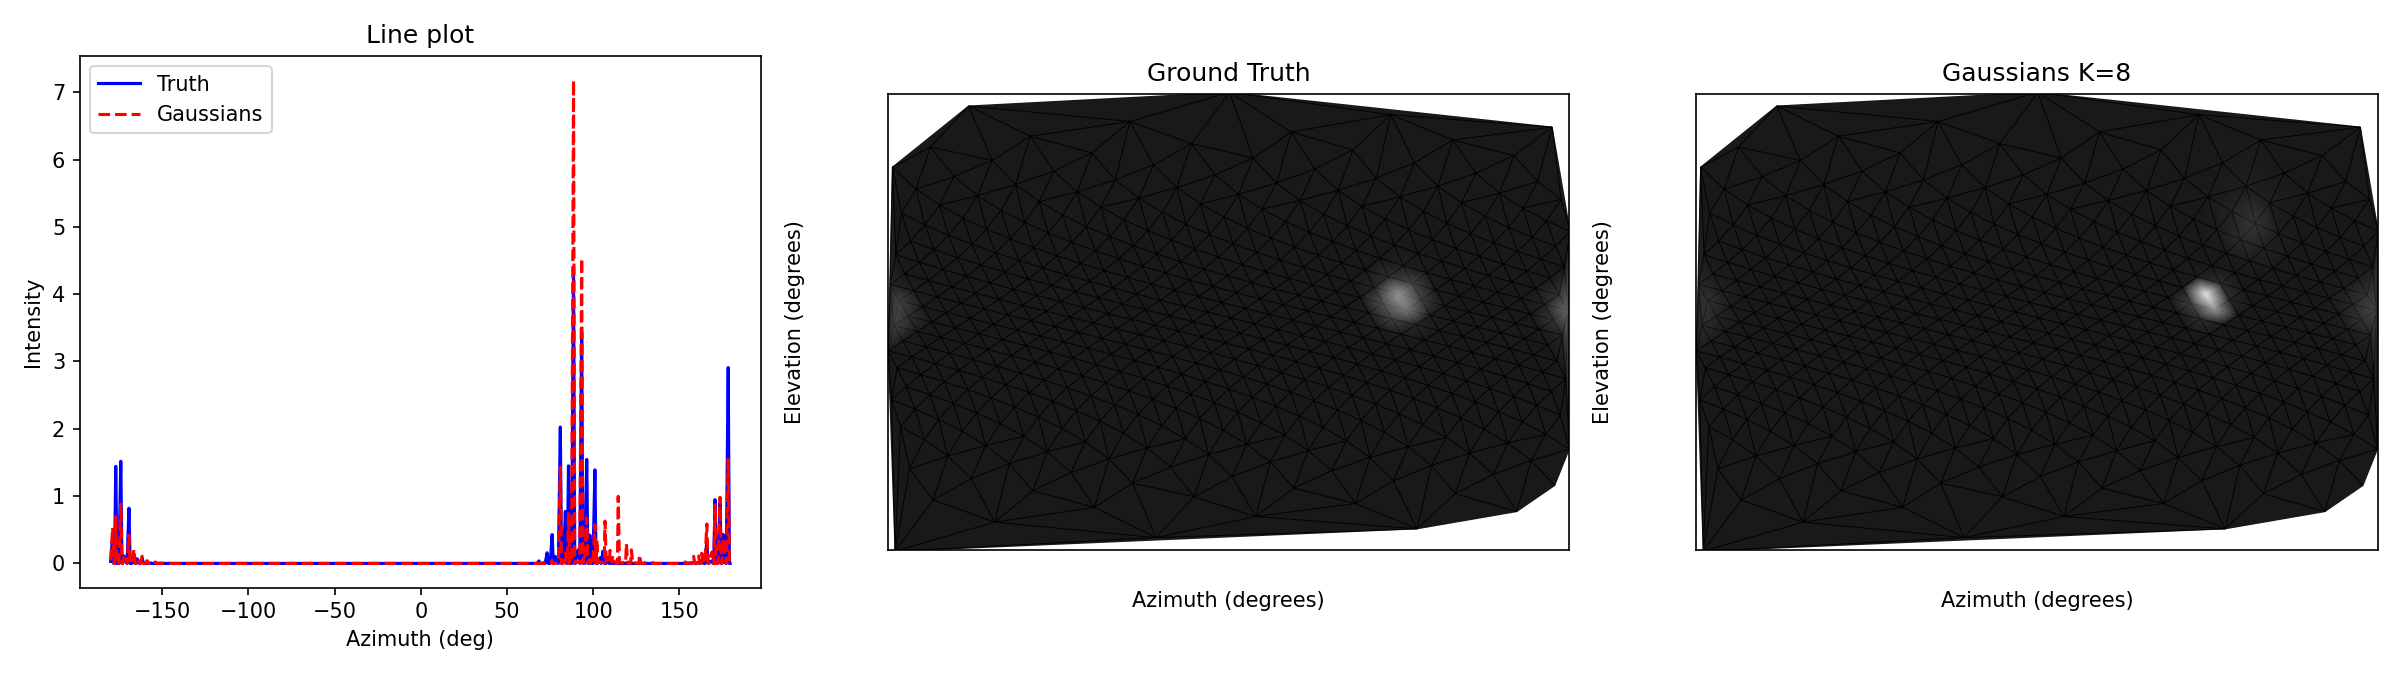
\includegraphics[width=\textwidth]{media/gauss_vs_truth.png}
\caption{Grid-based variant: azimuthal intensity profiles (left) and spherical Miller-projection maps (center: ground truth, right: Gaussian reconstruction).}
\label{fig:gauss_vs_truth}
\end{figure}

\begin{figure}[ht]
\centering
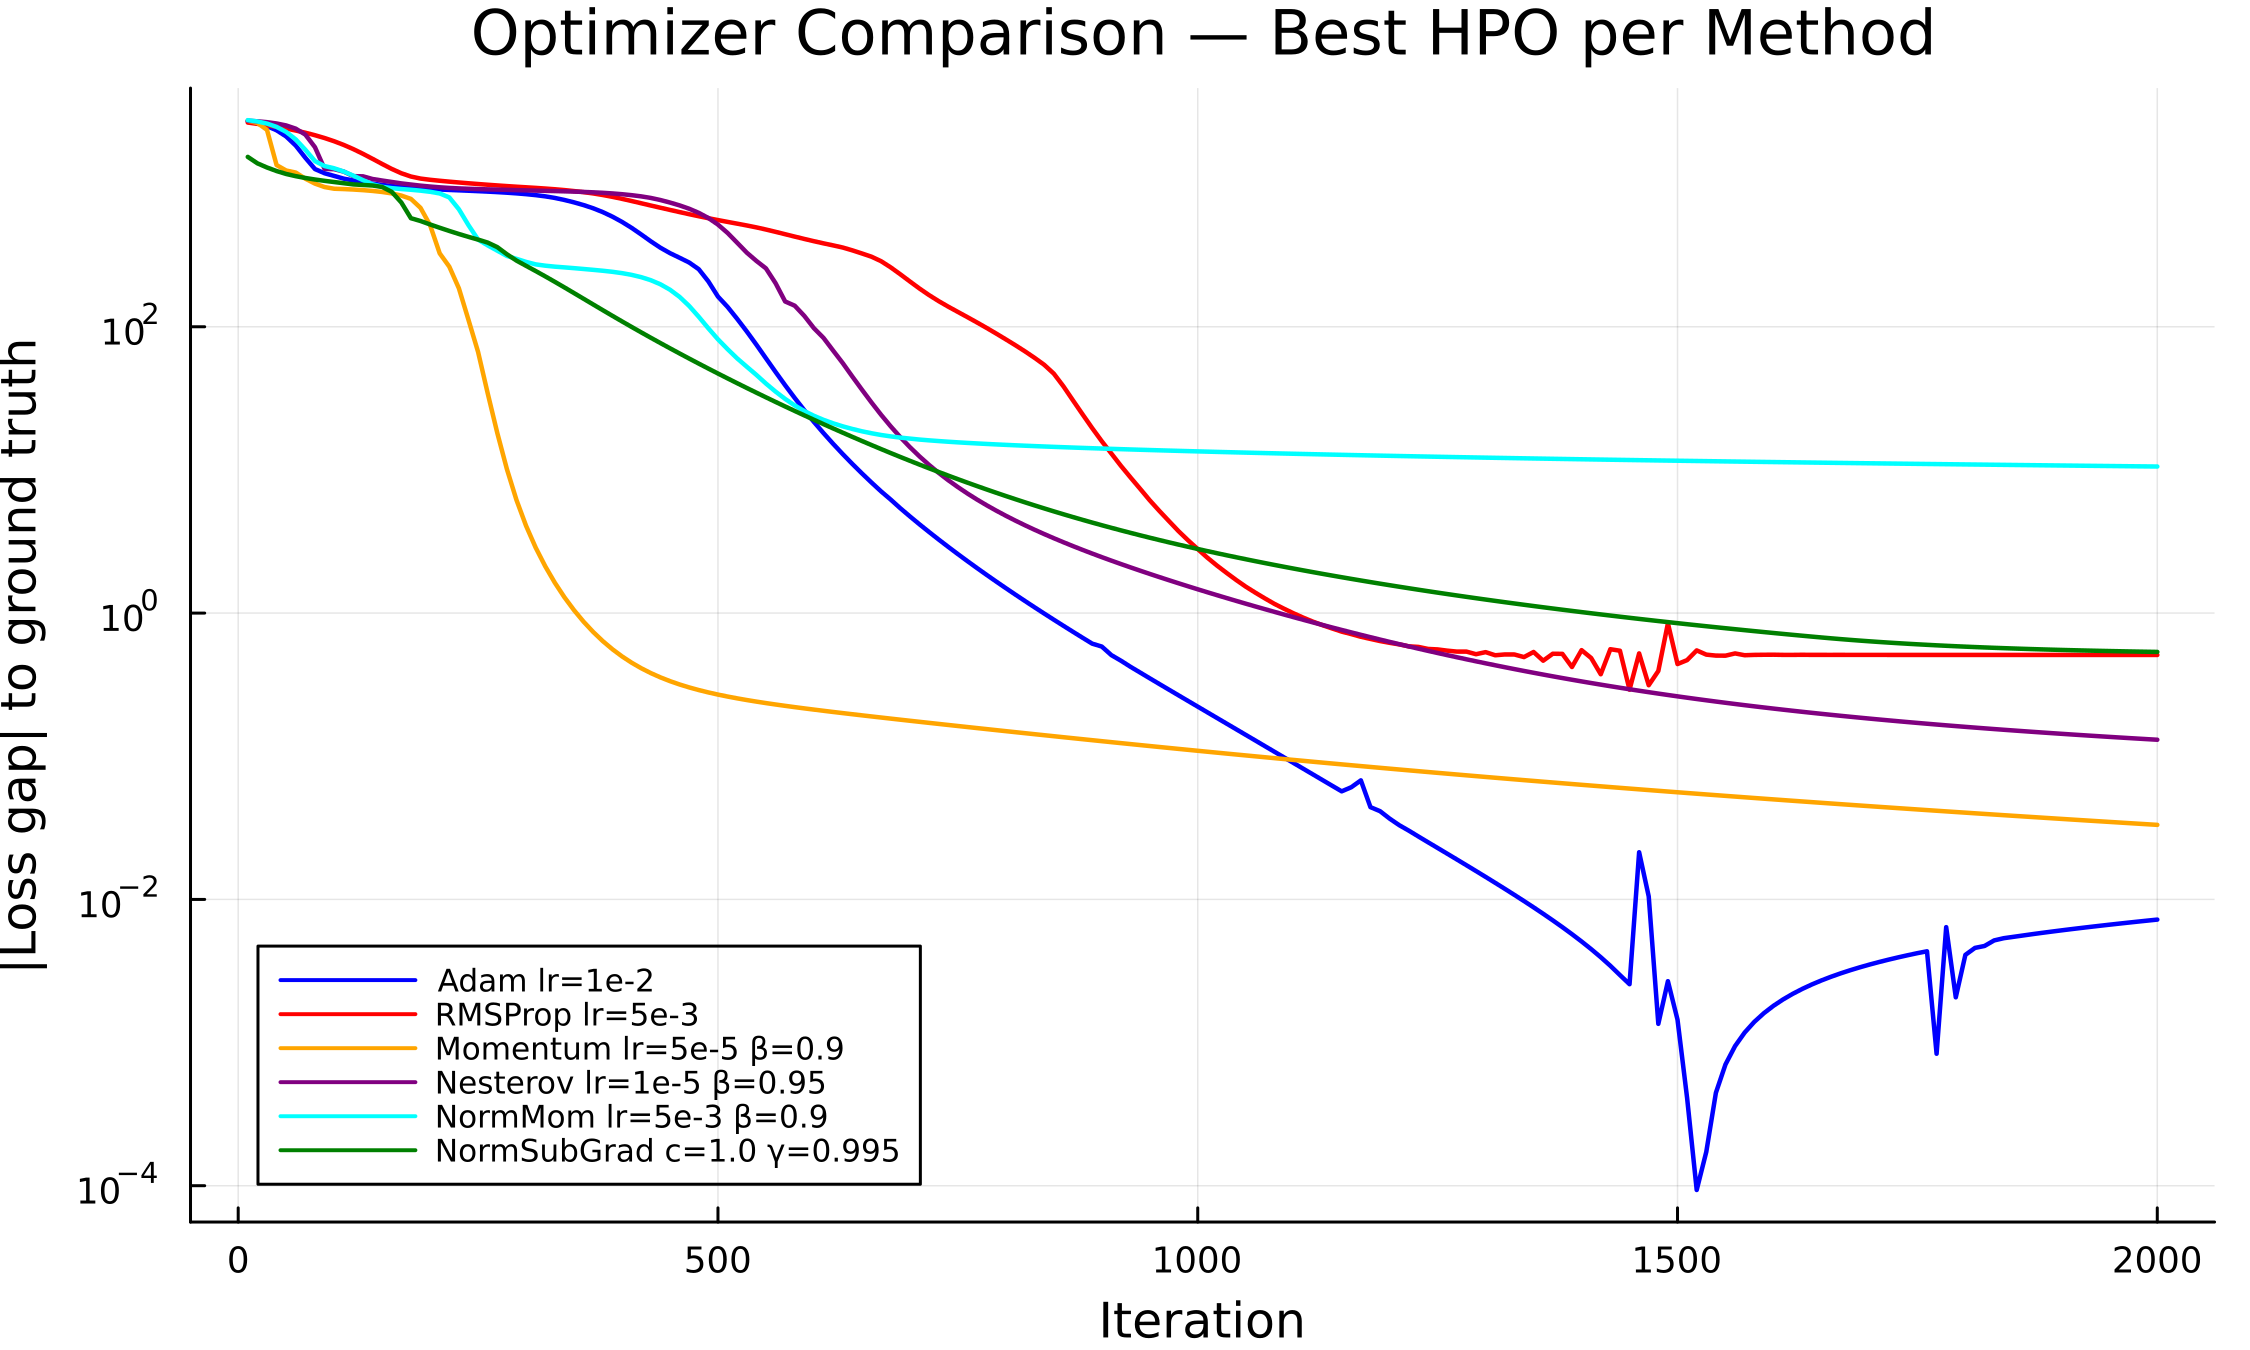
\includegraphics[width=0.85\textwidth]{media/optimizer_convergence.png}
\caption{Optimizer comparison on the grid-based variant (K=8, 2000 iterations). Adaptive methods (Adam, RMSProp) converge reliably; momentum requires a 200$\times$ smaller LR.}
\label{fig:optimizers}
\end{figure}

Six optimization methods were benchmarked (Figure~\ref{fig:optimizers}). The key challenge was ill-conditioning across parameter scales ($\mu_k \sim$ radians, $\pi_k$ spanning orders of magnitude), resolved by Adam's per-parameter adaptive learning rates.

\begin{figure}[ht]
\centering
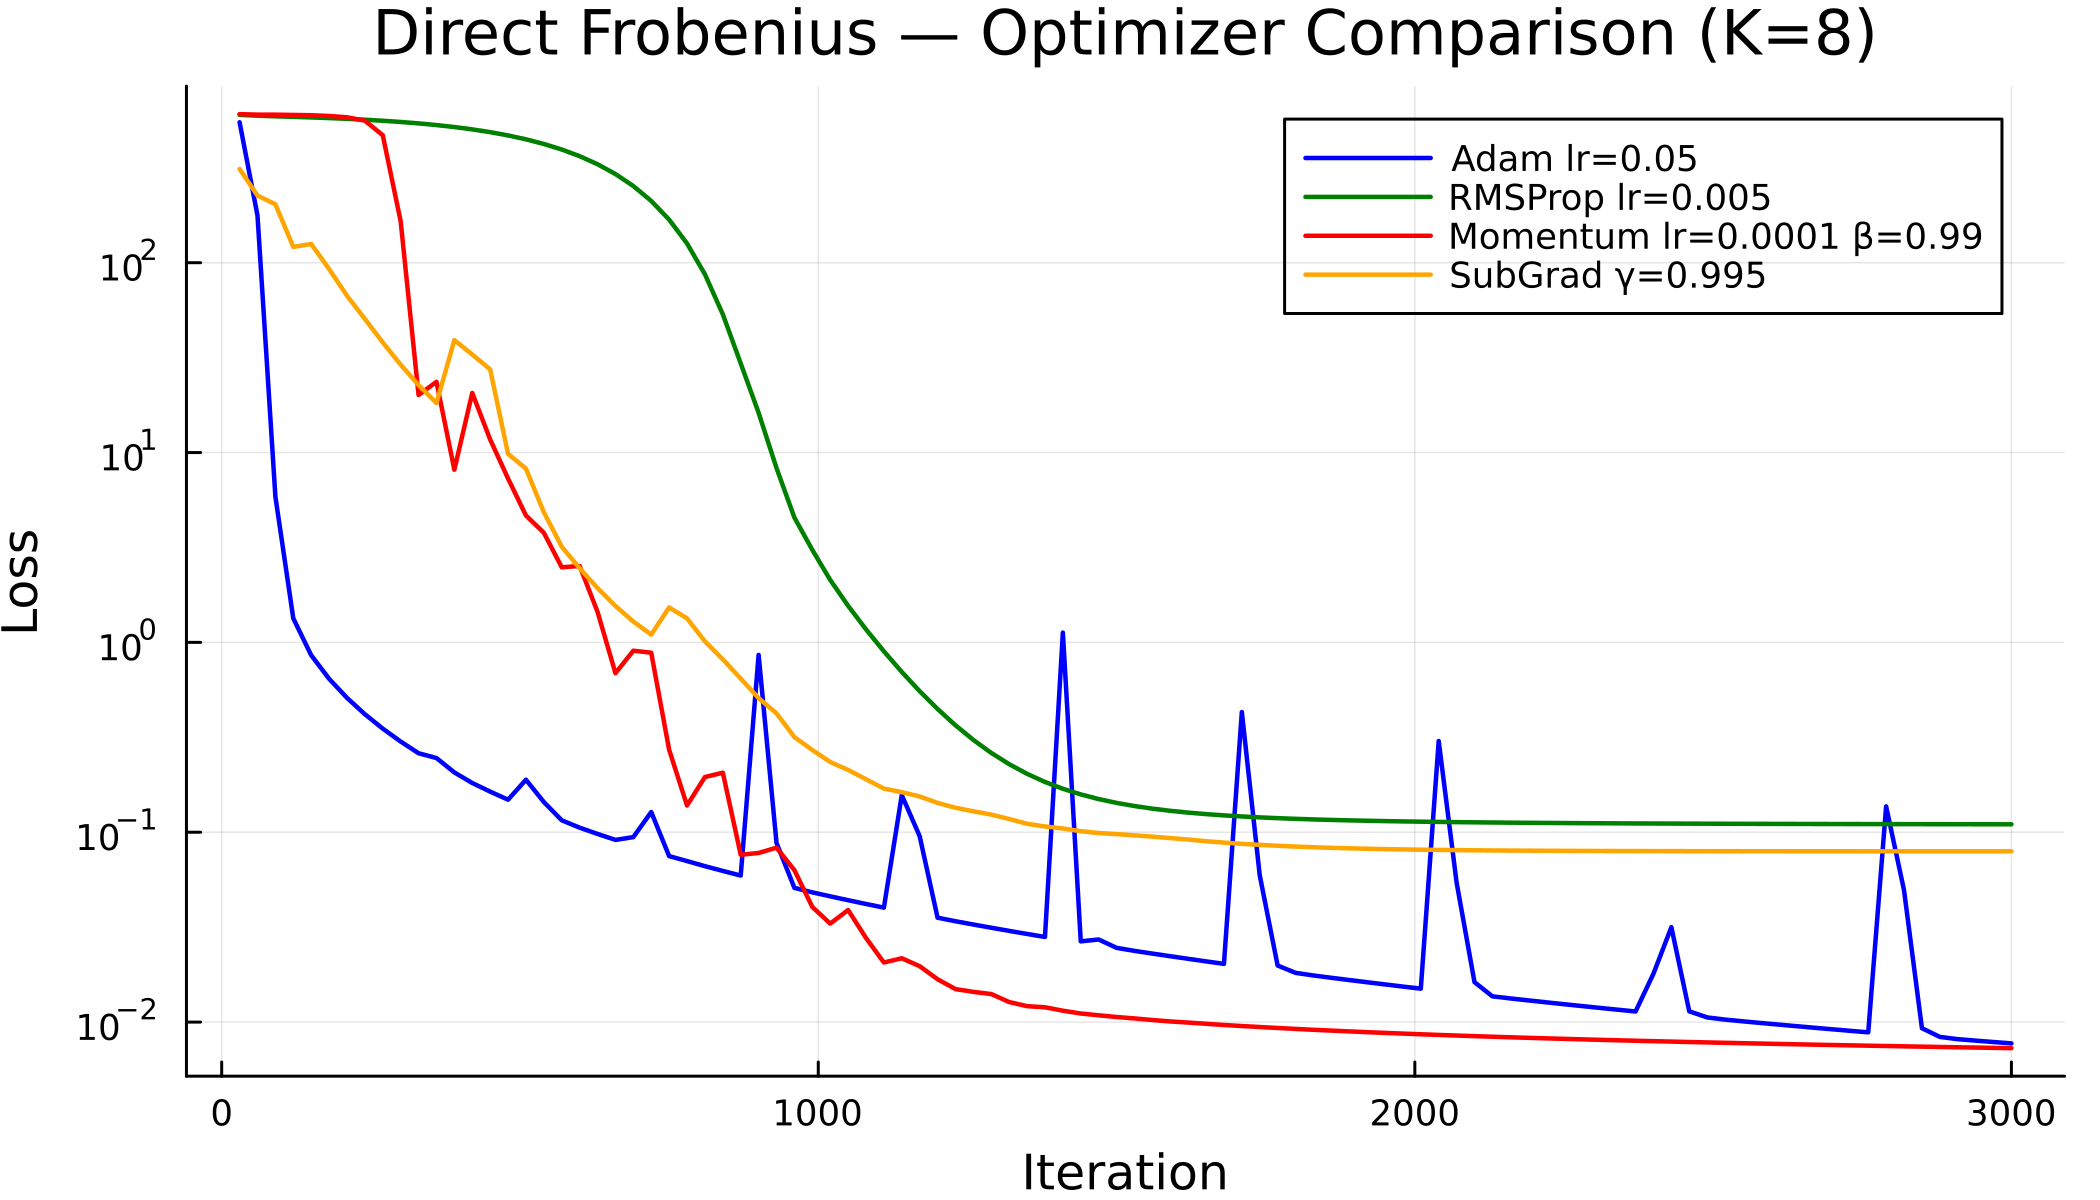
\includegraphics[width=0.85\textwidth]{media/direct_opt_compare.png}
\caption{Optimizer comparison on the direct covariance matching formulation (K=8, 3000 iterations). The better-conditioned loss landscape allows momentum to converge with a 10$\times$ larger learning rate than in the grid variant.}
\label{fig:direct_opts}
\end{figure}

The direct formulation's optimizer comparison (Figure~\ref{fig:direct_opts}) confirms that the $4\times 4$ covariance space is better conditioned than the 484-point grid.


\section{Wishart Log-Likelihood Alternative}
\label{sec:wishart}

The Frobenius loss treats all covariance entries equally. A principled alternative under the complex Gaussian measurement model is the Wishart negative log-likelihood:
\[
\mathcal{L}_{\text{Wishart}}(\Theta) = \log\det C_{\text{pred}}(\Theta) + \operatorname{tr}\!\big(C_{\text{pred}}^{-1}\,C_{\text{obs}}\big)
\]
with analytical gradients via matrix derivatives. Empirically, the Wishart loss achieved NMSE 1.06 at 44~$\mu$s/iter (3$\times$ slower due to the $4\times 4$ matrix inverse), performing worse than the Frobenius approximation (NMSE 0.40) on our synthetic test setup. The Frobenius loss is retained as the primary method for its speed-accuracy trade-off.

\begin{figure}[ht]
\centering
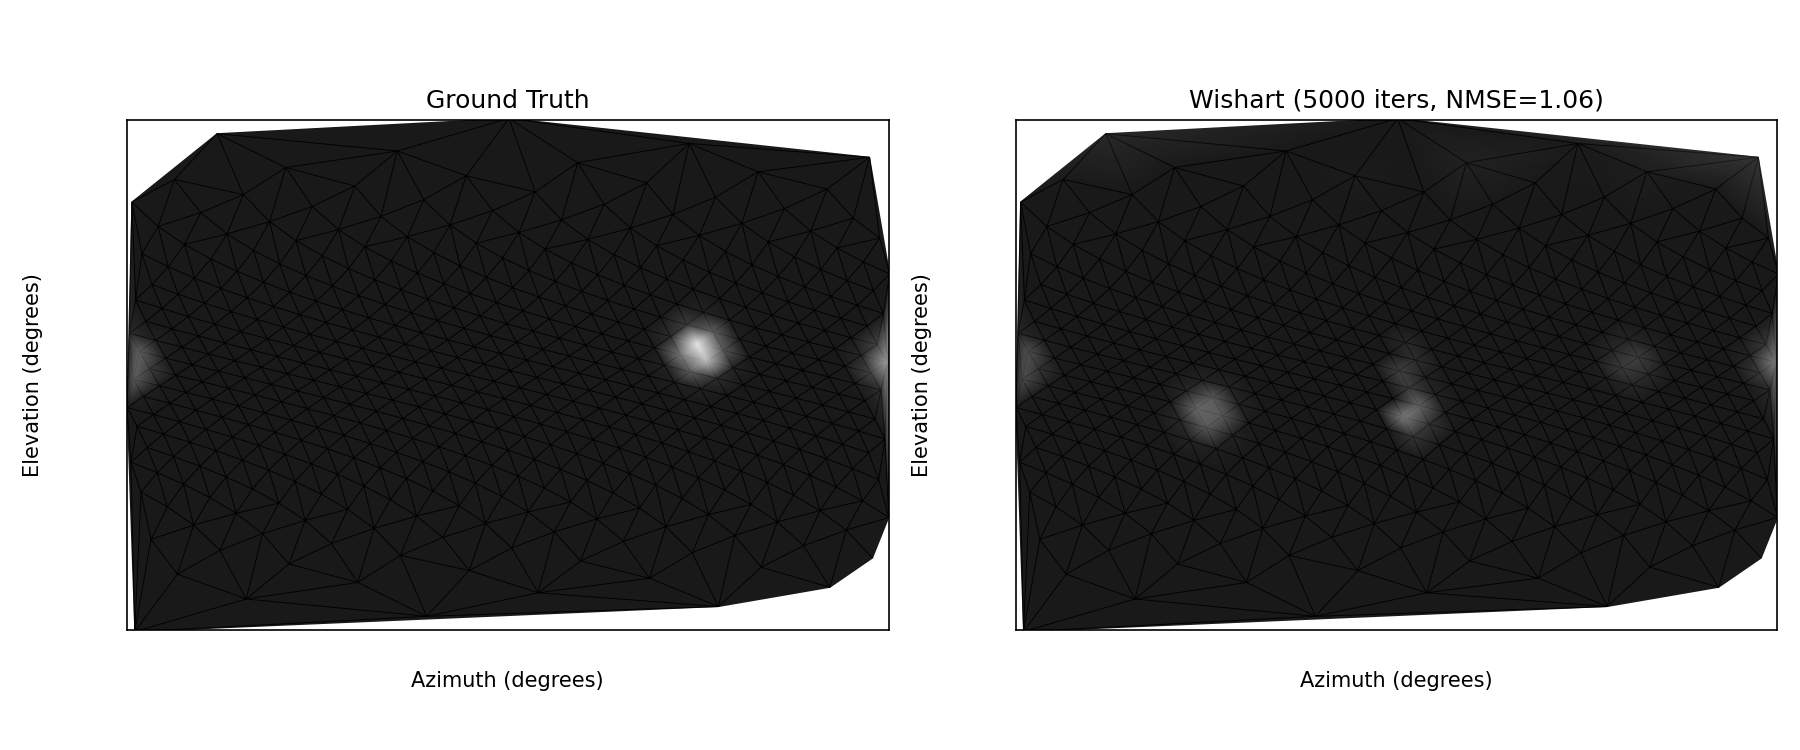
\includegraphics[width=\textwidth]{media/wishart_viz.png}
\caption{Wishart log-likelihood fit: ground truth (left) vs.\ fitted Gaussians (right). Sources partially recovered (NMSE 1.06).}
\label{fig:wishart}
\end{figure}


\section{Gauss-Newton Failure Analysis}
\label{sec:gn}

For the nonlinear least squares problem $\mathcal{L}_{\text{spatial}}$, we attempted a Gauss-Newton solver with Levenberg-Marquardt damping. The Jacobian $J \in \mathbb{R}^{32 \times 32}$ was validated analytically (error 0.0 against finite differences). However, the update $\Delta v = -(J^\top J + \lambda I)^{-1} J^\top r(v)$ consistently rejected all steps: the exponential nonlinearity in the steering vector $\mathbf{a}(\mu) = \exp(-i k \mathbf{r}\cdot\mathbf{s}(\mu))$ causes the linearized model to overshoot by $>2$~radians per step, even with heavy damping ($\lambda \rightarrow \infty$). At large $\lambda$, the method reduces to slow gradient descent, defeating its purpose. The 4-mic array spans approximately one full wavelength (85~mm at $\lambda \approx 70$~mm), so a 2-radian step moves the source through a complete steering vector oscillation---far outside the linear regime required by Newton-type methods.


\section*{Acknowledgments}

%Bibliography
\bibliographystyle{unsrt}  
\bibliography{references}  


\end{document}
